\p
با حالت‌بندی روی اولین نقطه ای که ریک دوباره به سطح زمین بر می گردد می‌توانیم به یک رابطه بازگشتی برسیم. تعریف می‌کنیم \(C_n\) حل مساله برای مسیر به طول n است. مدل حرکت ریک در شکل زیر آمده است. ریک از خانه زرد سمت چپ حرکتش را آغاز می‌کند و در هر حرکت یا به خانه بالا راست خانه فعلی و یا به خانه پایین راست خانه فعلی در صورت وجود می‌رود.
\begin{figure}[h!]
    \centering
    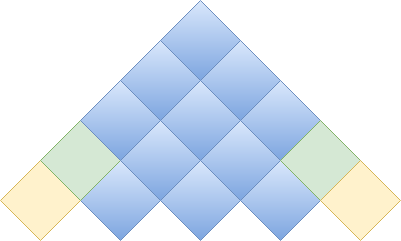
\includegraphics[width=0.2\linewidth]{DMsoal3.png}
    		\caption{مدل مساله}
\end{figure}
حال اگر ریک دوباره برای اولین بار در نقطه با طول i به زمین که خانه‌های پایین‌ترین سطر است، برگردد قبل آن قطعا در خانه‌ی بالا چپ آن قرار داشته است. فرض کنید اولین برخورد ریک به سطح زمین در شکل خانه ی زرد سمت راست باشد. در این صورت ریک حتما یک حرکت قبل در خانه سبز سمت راست قرار داشته است. همینطور ریک در ابتدای مسیر، حتما از خانه سبز در سمت چپ شکل عبور کرده است و در مسیر میان دو خانه سبز دیگر از سطح اول که زمین باشد عبور نکرده است زیرا می‌دانیم خانه زرد سمت راست، اولین فرود ریک در طی مسیر است، بنابراین می‌توان شرایط حرکت ریک بین دو خانه سبز را حل همین مساله برای حالت \(C_{i-1}\) دانست که حل مساله برای مثلث کوچکتر که از ارتفاع خانه‌های سبز شروع می‌شود است که با توجه به این که حالات حرکت بین دو خانه زرد با حالات حرکت بین دو خانه سبز یکی است، \(C_{i-1}\) برابر با تعداد حالات حرکت ریک تا اولین سقوطش نیز هست. بنابراین به رابطه زیر می‌رسیم که بر اساس فرود اول، حرکت ریک را حالت بندی می‌کند:
\[ C_n = \sum\limits_{i=1}^{n} C_{i-1}C_{n-i} \]طبق چیزی که در بالا دیدیم، از مسیر حرکت ریک، \lr{n-i} خانه پس از برخورد اول با زمین در خانه i ام باقی می‌ماند که جمله \(C_{n-i}\) را نتیجه می‌دهد. بنابراین به رابطه اعداد کاتالان رسیدیم و طبق فرمول بسته برای جواب این مساله داریم:
\[ C_n = \frac{(2n)!}{(n+1)!n!} \]که جواب مساله است.
  